%!TEX program = xelatex
%!TEX TS-program = xelatex
%!TEX encoding = UTF-8 Unicode

\documentclass[12pt, a4paper]{article} % A4 纸,字体大小为 12pt 的 article 类文档
\usepackage{CJKutf8} % 中文支持
\usepackage{graphicx} % 插入图片
\usepackage{subfigure} % 插入多图时用子图显示的宏包
\usepackage{listings} % 支持代码显示
\usepackage[colorlinks,linkcolor=blue]{hyperref} % 超链接
\usepackage{ulem} % 删除线
\usepackage{xcolor} % 定制颜色
\usepackage{caption2} % 浮动图形和表格标题样式
\usepackage{amssymb} % 数学符号
\usepackage{indentfirst} % 中文段落首行缩进
\usepackage{tikz} % 画图
\usepackage{pgfplots} % 画图
\usepackage{amsmath} % 处理数学公式
\usepackage{mathtools} % 处理数学公式
\setlength{\parskip}{0.5em} % 段落间距
\renewcommand{\figurename}{图} % 将图表的标题设置为中文“图”
\usetikzlibrary{tikzmark,calc,decorations.pathreplacing} % tikzmark 用于标记位置,calc 用于计算,decorations.pathreplacing 用于画大括号


\title{第十九·信号传递·信息不全如何进行博弈}
\author{hoochanlon}
\date{\today}

\begin{document}
	\begin{CJK*}{UTF8}{gbsn}
		\maketitle
        \clearpage
        \section{信息不对称}
        \subsection{信息不对称分类}
       是真文凭、假文凭,对方不知道;网上下单,对课程、书籍质量不了解;入职以后真努力还是假努力,老板不清楚;这就存在信息不对称。

       \[
        \text{信息不对称的分类}
        \begin{cases}
             \text{时间}\left\{
                \begin{aligned}
                    &\text{事前的信息不对称}  \\
                    &\text{事后的信息不对称}
                \end{aligned}
             \right. \\
             \text{内容}\left\{
                \begin{aligned}
                    &\text{关于行动的}  \\
                    &\text{关于信息(或知识)的}
                \end{aligned}
             \right.
        \end{cases}
    \]

    \subsection{信息不对称的博弈}

    注意:事情还没发生,还没开始,只能是事前隐藏信息,而没法隐藏行动。研究事前隐藏信息的模型,我们叫逆向选择的模型,研究事后不对称信息的模型,我们叫道德风险模型。
        \begin{itemize}
        \centering
        \item[] ~~~~~~~~~~~~~~~~~~~~~~~~事前隐藏信息 —— 逆向选择模型 \tikzmark{a}
        \item[] 事后隐藏信息~ \tikzmark{b}
        \item[] \sout{事前隐藏行动}~ \tikzmark{c}
        \item[] 事后隐藏行动~ \tikzmark{d}
        \end{itemize}
        \begin{tikzpicture}[remember picture,overlay]
        \draw[line width=1pt,decorate,decoration={brace,amplitude=10pt}]({pic cs:c} |- {pic cs:b}) +(0,1em)
        -- node[right,inner sep=1.5em] {道德风险模型} ({pic cs:b}|- {pic cs:d});
        \end{tikzpicture}

    信号传递和信息甄别的区别:
    \begin{itemize}
        \item 拥有优势的一方先行动为\textbf{信号传递}。
        \item 拥有信息劣势一方先行动为\textbf{信息甄别}。
    \end{itemize}
    信号传递的首要目的就是“我是谁”,信息甄别的目的“你到底是谁”。

    \clearpage
    \section{贝叶斯法则}
    贝叶斯定理,是概率统计中的应用所观察到的现象对有关概率分布的主观判断(先验概率)进行修正的标准方法。是指当分析样本大到接近总体数时,
    样本中事件发生的概率将接近于总体中事件发生的概率。\par
    \begin{itemize}
        \item[] 假设:P(A)是A发生的概率
        \item[] ~~~~~~~~~P(B)是B发生的概率
        \item[] ~~~~~~~~~$P(A|B)$是B发生的条件下A发生的概率
        \item[] ~~~~~~~~~$P(B|A)$是A发生的条件下B发生的概率
    \end{itemize}
    贝叶斯法则作用:通过已知的三个概率来算出未知的第四个概率。

    \begin{align*}
        P(A \cap B) &= P(A) \times P(B|A) = P(B) \times P(A|B) \\
        \\
        P(A|B) &= \frac{P(A) \times P(B|A)}{P(B)}
    \end{align*}

    \subsection{贝叶斯法则的应用}
    一班同学50个人,30个男生,20个女生;15男同学选择博弈论课程,16个女女同学选择博弈论课程。一个选择博弈论课程的同学,他是男生的概率是多少?
    \begin{itemize}
        \item[]  假设:A代表男生,$P(A)=0.6$;B代表选择博弈论课程,$P(B|A)=0.5$
        \item[] ~~~$P(B)=P(A) \times P(B|A)+(1-P(A) \times 0.8)=0.62$
        \item[] ~~~$P(A|B)=\frac{P(A) \times P(B|A)}{P(B)}=\frac{0.6 \times 0.5}{0.62}=48.38\%$
    \end{itemize}
    在不完全信息的动态博弈中,因为需要分析参与者如何根据信息的变化,来调整信念并改变行为的整个全过程,那么贝叶斯法则的作用就产生了。
    不完全信息的静态博弈的纳什均衡,就是贝叶斯均衡。不完全信息动态博弈的纳什均衡,叫做完美贝叶斯纳什均衡。

    \clearpage
    \section{信号传递博弈}
    \begin{itemize}
        \item[] 假设:参与人1是信号的发送者,类型是私人信息。
        \item[] ~~~~~~~~~~参与人2是信号的接收者,类型是共同知识。
    \end{itemize}
    \begin{itemize}
        \item "自然"首先选择参与人1的类型。
        \item 参与人1选择发送信号。
        \item 参与人2在观测参与人1发出的信号后,把先验概率转化为后验概率,然后选择其相应的行动。
    \end{itemize}
    你的信息传递会改变我对你的类型判断,这一点参与者1他事先也是能预期到的,参与者1在发信号的时候,他也能预期到参与者2会这么做。当双方结束以后,
    那么再根据损益函数,获得各自的博弈结果。\par
    参与者1在发信号的时候,他是能够事先预测到参与者2将根据他发的信号,来修正对他类型的判断。因此他会选择一个对他自己来说最优的叫类型依存的信号。
    当然参与者2也知道参与者1已经考虑到他的信息效应。

    \subsection{进入市场博弈}
    \begin{figure}[htbp]
        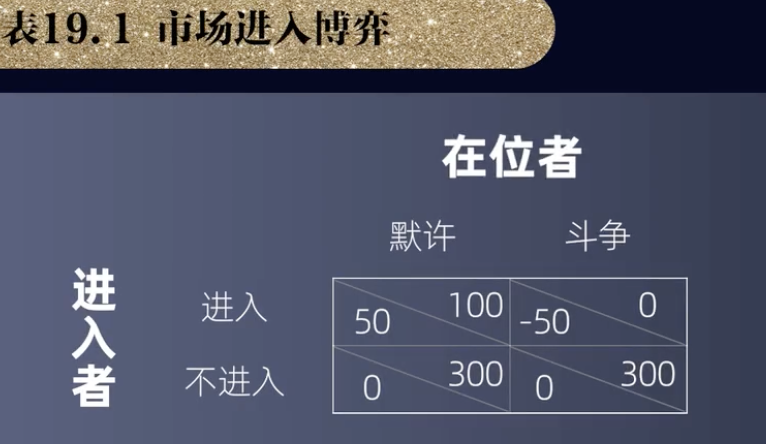
\includegraphics[width=1\textwidth]{./figures/catch2023-08-03-17.17.25.png}
    \end{figure}
    在位者选择斗争的话,进入者不但赚不到钱反而亏了,当然在位者也没了收益。进入者是否进入,取决于就是我一旦进来后,在位者会不会跟我斗。
    那么对于在位者来说,他当然不希望对方进来。威胁不可信,因为它不构成子博弈的纳什均衡。\par

    那么假设在位者是两种类型,高成本与低成本,如下图:
    \begin{figure}[htbp]
        \centering
        \subfigure[高成本型]{
            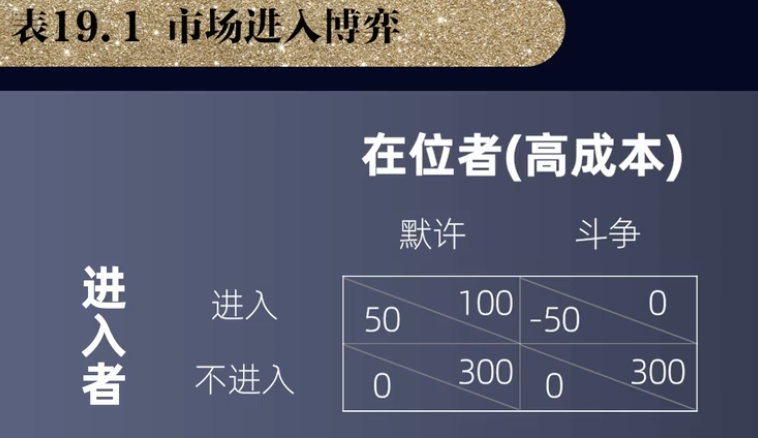
\includegraphics[width=0.46\textwidth]{./figures/catch2023-08-03-17.26.20.png}
        }
       \subfigure[低成本型]{
            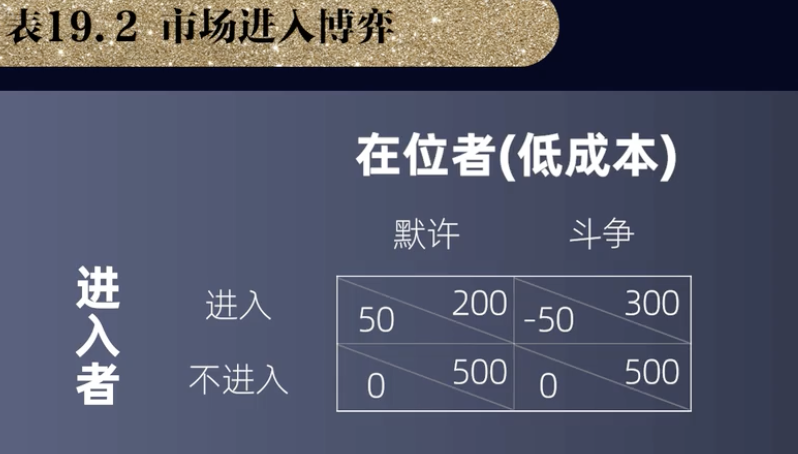
\includegraphics[width=0.46\textwidth]{./figures/catch2023-08-03-17.27.18.png}
        }
    \end{figure}
    斗争的收益,大于默许的收益。那么对于进入者来说,他是否选择进入,不是因为成本关系,而是取决于在位者类型,这样绑架博弈是一样的。由于信息不对称,
    它只能根据对对方的类型的信念(先验概率)做选择。\par
    要是进入者误以为在位者是低成本的,实际上进入后发现是高成本的,导致两方收益下降。那么在位者一方就需要发出对低成本进入者的警告信号。这样的话,
    关于他的类型是一个真实的信息,然后对方相信这个类型以后他就不进来,那我可以获得更高的收益。

    光是说“我是高成本的,你别进来”这没用。因为不管高低成本的在位者都会这么说,因为进入者不进来,收益最大。问题来了,那我怎么又相信你的话呢?
    比方说:在位者产品定价作为他生产成本的信号,低成本的在位者定一个很低的价格,低到高成本的在位者没有能力来模仿你,想假装都假装不了。
    那么就会改变对事物的认知。

    \clearpage
    \section{信息传递}

    \subsection{信息传递的类型及结论}

    \[
        \text{信息传递的均衡类型}
        \begin{cases}
             \text{分离均衡}\left\{
                \begin{aligned}
                    &\text{不同类型的发送者选择不同的信号,} \\
                    &\text{信号准确地揭示出参与者的不同类型。} \\
                    &\text{例如:好人做好事,坏人做坏事。}
                \end{aligned}
             \right. \\\\
             \text{混同均衡}\left\{
                \begin{aligned}
                    &\text{不同类型的发送者选择相同的信号,} \\
                    &\text{接受者还是根据一开始的先验概率来抉择。} \\
                    &\text{例如:大家都会做,好人坏人都会做。}
                \end{aligned}
             \right. \\\\
             \text{准分离均衡}\left\{
                \begin{aligned}
                    &\text{某些类型的参与者随机地发送信号,}  \\
                    &\text{另一类参与者选择特定的信号。} \\
                    &\text{例如:好人会做,坏人可能做,可能不做}
                \end{aligned}
             \right.
        \end{cases}
    \]

    博弈的结果是混同还是分离均衡,跟参与者的先验概率是有关系的。如果你一开始认为世界好人多,你就相信对方是好人;如果你认为世界上还是坏人多,除非
    对方做了足够好的事情,你才愿意相信他是好人。很多时候的行为选择跟你的先验概率是关系的,哪怕你做调整,也跟你一开始怎么认为是有关系的。\par

    信号之所以能起到参与人传递类型的作用,是因为参与者的行为是类型依赖的。他怎么做跟他什么样的人是关系的。所以我们之所以能够通过“观其言察其行”来
    推测一个人的类型,就是因为言行和类型是相关的。每个参与者传递信号的能力,或者成本差异,是信号传递能够起作用的根本原因。或者从另外一个角度说,
    就是信息不对称逼迫信息优势的这一方,不得不花费一定代价,来证明自己的类型。 \par

    \end{CJK*}
\end{document}
